\section{Introduction}

% \input{Main_Text/Figures/teasar}

\begin{figure}
    \centering
    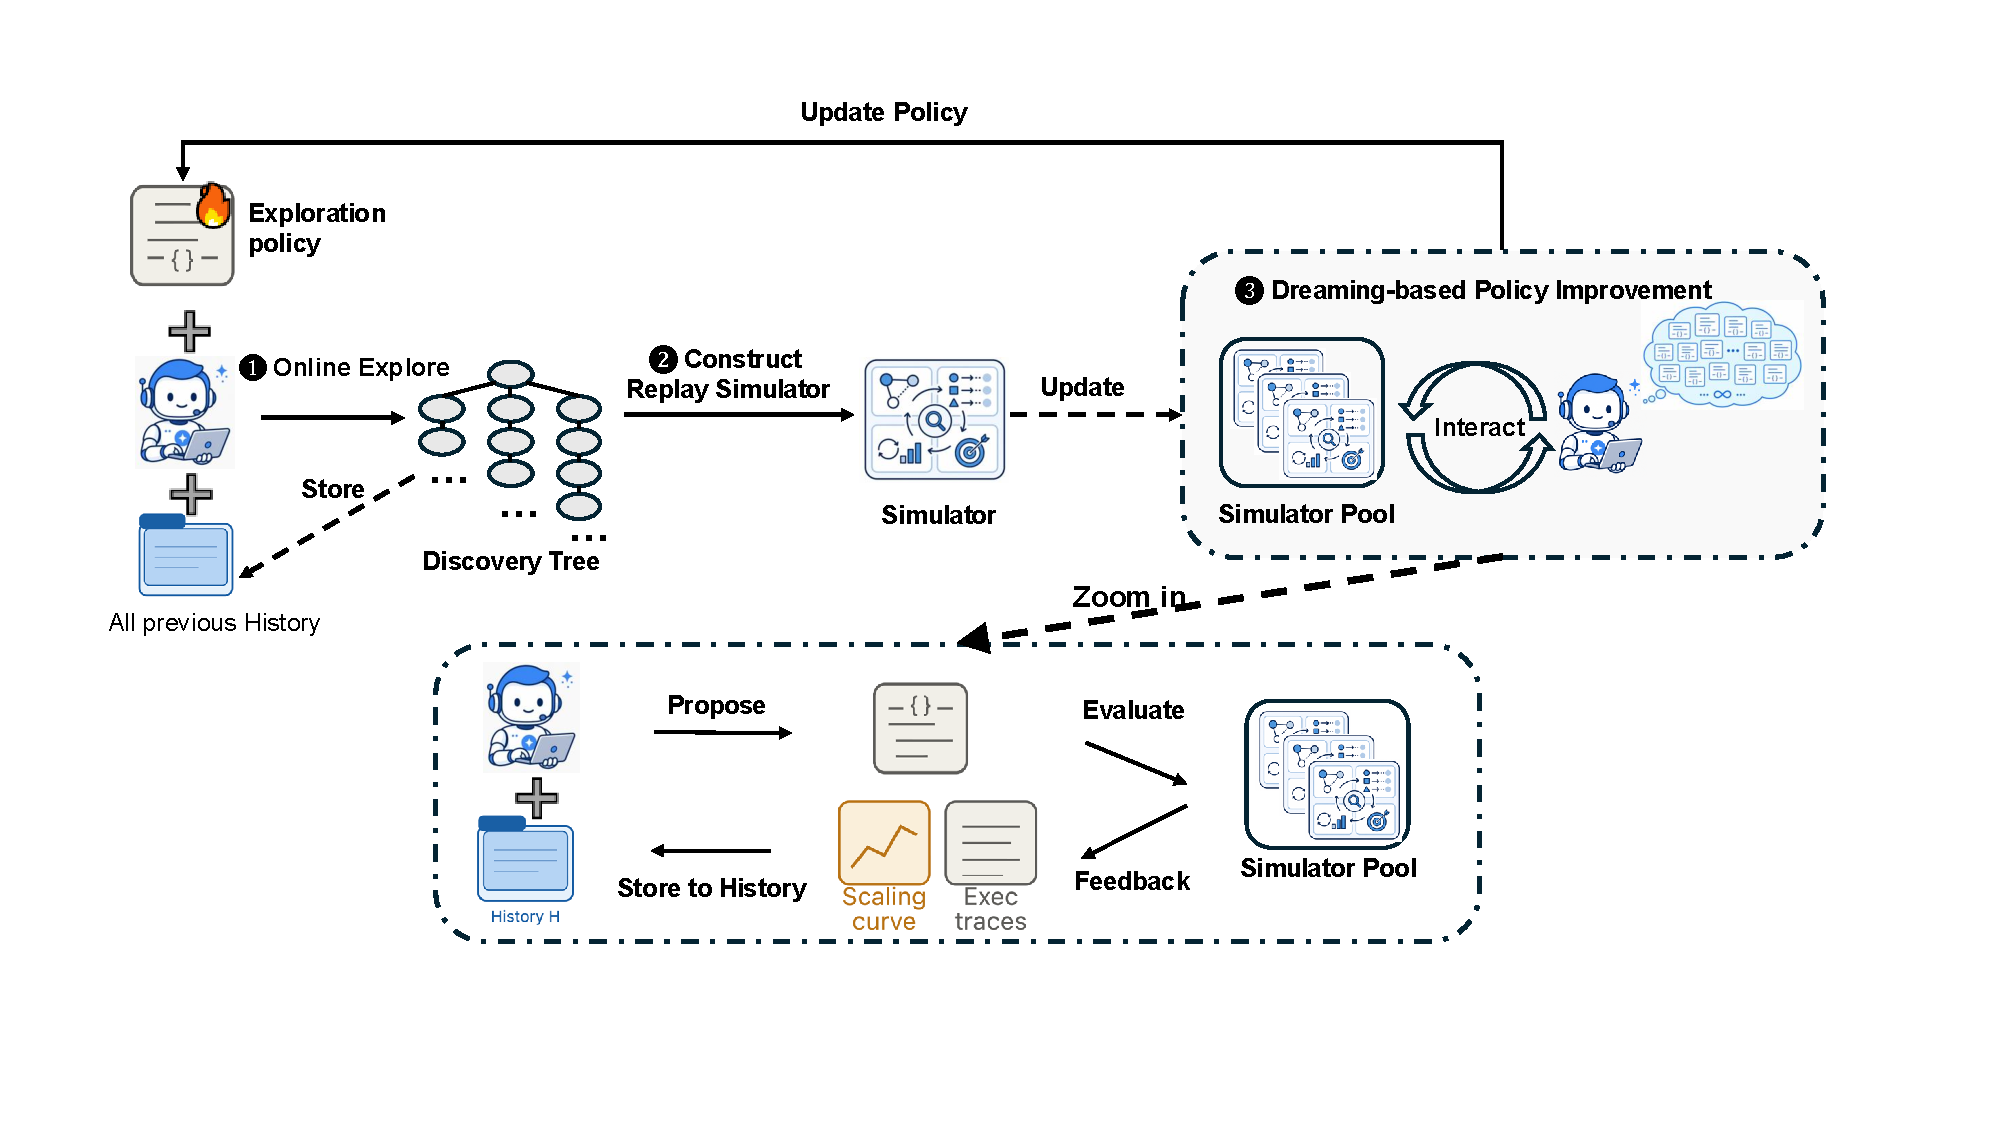
\includegraphics[width=0.93\linewidth]{Main_Text/Figures/Dream-RSI-latest.pdf}
    \caption{\textbf{Overview of \textsc{Dream-RSI}.} The system operates in a recursive self-improvement loop via three core stages: \textbf{\textcircled{1} Online Explore}, where the current exploration policy guides a coding agent to expand a discovery tree and log historical traces; \textbf{\textcircled{2} Construct Replay Simulator}, where the generated discovery tree is converted into a reusable simulator pool; and \textbf{\textcircled{3} Dreaming-based Policy Improvement}, where the agent "dreams" up a massive pool of alternative policies in its mind. It then feeds these candidate policies into the replay simulator to simulate executions and derive rapid feedback, continuously refining its strategy (detailed in the Zoom-in box). The updated policy then redeploys for the next round of online exploration.}
    \label{fig:method}
\end{figure}


Recursive self-improvement (RSI) has emerged as an ambitious goal for autonomous AI systems~\citep{202608.0051}. A common mechanism underlying RSI is an iterative discovery loop wherein agents generate candidate solutions, evaluate outcomes, incorporate feedback, and refine future iterations. Such discovery loops have driven substantial progress across scientific and algorithmic domains, including algorithm design~\citep{novikov2025alphaevolve,romera2024mathematical}, open-ended mathematical optimization~\citep{georgiev2025mathematical,anthropic2026riemann}, systems design~\citep{jaber2026autokernel,cao2026k}, and agent self-improvement~\citep{zhang2026darwin,zhang2026hyperagents,lee2026meta,zheng2026llms}, with these discoveries increasingly feeding into the development of more capable AI systems. As agent capabilities improve and self-improvement targets become challenging, discovery increasingly requires long-horizon exploration over vast search spaces, often spanning thousands of proposal--evaluation cycles~\citep{ye2026evaluation,openai2026navierstokes}. At this scale, the ability to orchestrate exploration becomes critical~\citep{zheng2026parallel}. Poor exploration can waste substantial computation and time, severely limiting the efficiency and scalability of RSI.

Existing approaches have largely relied on manually designed exploration strategies that remain largely fixed throughout discovery~\citep{novikov2025alphaevolve,yan2026pacevolve,du2026mlevolve,jiang2026deltaevolve,ye2026evaluation}. Fixed strategies cannot improve from accumulated discovery experience and may repeatedly allocate computation to ineffective search directions.  Recent work therefore seeks to optimize exploration policies online during discovery~\citep{liu2026evox}, but doing so faces two fundamental bottlenecks. First, feedback is delayed and expensive at the meta level: unlike evaluating an individual candidate, assessing an exploration policy requires observing how it shapes the subsequent discovery process over many proposal--evaluation cycles. Second, the meta-policy space is vast: a newly proposed policy may perform poorly, so many alternatives may need to be tried. Together, these challenges make meta-level improvement particularly costly: each policy may require a long online rollout before receiving useful feedback, making it difficult to efficiently close the self-improvement loop at the exploration layer. 

To address these bottlenecks, our key intuition is simple: a fast and inexpensive simulator of discovery would allow many exploration policies to be evaluated before costly online deployment. \textbf{Surprisingly, completed discovery histories already provide such a simulator.} While prior work treats past discovery history merely as static textual context~\citep{hu2025memory,ouyang2026reasoningbank} or training data for weight fine-tuning~\citep{yuksekgonul2026learning,wang2025thetaevolve}, a completed discovery process inherently records a structured tree of past exploration decisions and their realized code-execution outcomes. Drawing an analogy to model-based reinforcement learning and World Models~\citep{ha2018world,hafner2023mastering} (\S\ref{sec:history_environment}), once organized into a discovery tree, this history can serve as a \textbf{replay simulator}~\footnote{We use the terms replay simulator and worlds interchangeably.}. As illustrated in Figure~\ref{fig:motivation}, an alternative exploration strategy can navigate this pre-recorded tree to traverse different subsets of recorded branches, in different orders, with different parallel groupings and stopping decisions. Because all execution outcomes are already saved in the tree, evaluating a new strategy requires only reading past records without rerunning the underlying discovery agent or evaluator. This transforms meta-policy improvement from an expensive online trial-and-error process into a fast, simulation-based ``dreaming'' procedure.

Building on this insight, we introduce \textsc{Dream-RSI}, a framework for scalable and recursively self-improving meta-exploration in agent-driven discovery. We first make exploration explicit and programmable through a lightweight orchestration layer that controls branching, parallel exploration, and stopping while leaving the underlying coding agent unchanged. Rather than keeping this policy fixed, \textsc{Dream-RSI} establishes a closed-loop self-improvement mechanism across three core stages (Figure~\ref{fig:method}): \textbf{(1) Online Exploration}, where the current policy guides real-world discovery and logs historical execution traces; \textbf{(2) Simulator Construction}, where recorded discovery trees are converted into a reusable replay simulator pool; and \textbf{(3) Dreaming-based Policy Improvement}, where candidate policies are evaluated via low-cost "dreaming" over the simulator. The updated policy is then redeployed online to generate new discovery experience and expand the simulator pool, closing a RSI loop at the meta-exploration layer.

Empirically, we evaluate \textsc{Dream-RSI} across 8 scientific discovery tasks spanning three distinct domains: algorithm engineering, mathematical optimization, and GPU kernel engineering. In algorithm engineering (Lasso path solver), \textsc{Dream-RSI} outperforms standard libraries like \texttt{sklearn} and strong baselines while reducing agent calls by up to $162\times$ over \textsc{SimpleTES} and $1.7\times$ over fixed-exploration baselines. In mathematical optimization (sum-difference, autocorrelation, circle packing), it matches or surpasses strong baselines within $1\text{k}$ generations, yielding over $50\times$ budget savings compared to \textsc{SimpleTES}. In GPU kernel engineering (KernelBench), it either reaches target execution speeds using $1.79\times$--$2.43\times$ fewer generations or improves kernel performance by up to $2.09\times$ under identical budget constraints.  

In summary, our main contributions are as follows: 1) \textbf{History as Replay Simulator:} We conceptualize completed discovery histories as replay simulators. This makes delayed exploration feedback reusable for efficient meta-exploration policy evaluation.;   2) \textbf{Meta-Layer RSI Loop (\textsc{Dream-RSI}):} We introduce \textsc{Dream-RSI}, establishing a recursive self-improvement loop that continuously collects discovery histories through online exploration, constructs replay simulators from history to refine meta-exploration strategies via  dreaming, and redeploys the upgraded policy online; 3) \textbf{Empirical Validation:} We conduct experiments to demonstrate that \textsc{Dream-RSI} improves both discovery effectiveness and efficiency in several settings.

